\documentclass[conference]{IEEEtran}
\usepackage{amsmath,graphicx,booktabs,array,url}
\urlstyle{same}
\title{Reliability-Gated Adaptive Sensing for Fault-Resilient Human Activity Recognition in Wearable IoT}
\author{
\IEEEauthorblockN{Anusuya M}
\IEEEauthorblockA{\footnotesize
\textit{School of Computer Engineering}\\
\textit{Manipal Institute of Technology, MAHE}\\
Manipal, Karnataka, India\\
Reg. No.: 240953480\\
\url{anusuya.mitmpl2024@learner.manipal.edu}}
\and
\IEEEauthorblockN{Vemba Kumar R}
\IEEEauthorblockA{\footnotesize
\textit{School of Computer Engineering}\\
\textit{Manipal Institute of Technology, MAHE}\\
Manipal, Karnataka, India\\
Reg. No.: 240953502\\
\url{vemba.mitmpl2024@learner.manipal.edu}}
\and
\IEEEauthorblockN{Tailam Praneeth}
\IEEEauthorblockA{\footnotesize
\textit{School of Computer Engineering}\\
\textit{Manipal Institute of Technology, MAHE}\\
Manipal, Karnataka, India\\
Reg. No.: 240953532\\
\url{tailam.mitmpl2024@learner.manipal.edu}}
}
\begin{document}
\maketitle
\begin{abstract}
Wearable human activity recognition (HAR) faces missing, noisy, biased, and frozen sensor streams while continuous multi-device sensing incurs acquisition and communication costs. We implement per-IMU classifiers, observable quality indicators, reliability-weighted probability fusion, and a controller that selects the next sensing window's active IMUs. Eight-subject leave-one-subject-out evaluation on official PAMAP2 six-class data gave adaptive random-forest clean observed-label macro-F1 $0.8574\pm0.0861$ at normalized sensing-cost proxy 0.5281. All-sensor uniform fusion gave $0.8891\pm0.0726$ at cost 1.0; a fixed wrist-plus-chest pair gave $0.9150\pm0.0482$ at cost 0.667. Under moderate wrist dropout, adaptive macro-F1 was 0.7919 versus 0.8501 for all-sensor uniform fusion. A subsequent inner-validation search selected a larger forest in six folds and changed the policy in three, but its held-out fixed-six-class clean macro-F1 was 0.8227 versus 0.8428 for the original configuration replayed under the same metric. The original policy reduced a simulated acquisition/communication cost proxy by 47.2\%; neither configuration improved recognition over the strongest fixed comparator. Hardware energy and clinical performance remain unmeasured.
\end{abstract}
\begin{IEEEkeywords}wearable IoT, human activity recognition, adaptive sensing, sensor reliability, reproducibility\end{IEEEkeywords}
\section{Introduction}
The Internet of Things connects sensors, gateways, and applications. AI-enabled IoT adds local inference to turn measurements into decisions. Body-worn devices make continuous activity monitoring possible, but practical streams can contain missing packets, sensor failures, and noise. Reliability-aware fusion can protect decisions after acquisition; it does not undo the acquisition cost. The research question is whether observable sensor health, HAR uncertainty, and an explicit sensing budget can guide the configuration used in the \emph{next} window. This implementation contributes a reproducible controller and evaluation protocol, without claiming a new fusion algorithm or measured hardware energy benefit.

In the intended deployment (Fig.~\ref{fig:architecture}), each inertial measurement unit (IMU) acquires local motion channels and sends a window or features to a nearby gateway. The gateway runs a compact activity classifier, combines available sensor predictions, and issues a control command before the next window starts. A cloud service could receive selected summaries for longitudinal monitoring, but the present experiment implements neither a cloud backend nor a physical wireless protocol. The pre-acquisition control command is the architectural element that could change future sampling and transmission volume. Probability fusion alone acts after acquisition and cannot claim the same effect.

The fault model is important because high activity recognition accuracy on clean prerecorded data says little about a failed node. A wrist IMU may become unavailable, a wireless interval may be absent, or a channel may freeze or drift while still transmitting plausible numbers. Treating every received value as equally credible risks allowing corrupted readings to dominate a decision. Equally, permanently retaining all three devices sacrifices the opportunity to reduce the number of measurements. These tensions motivate a joint evaluation of recognition, fault detection, and a clearly labeled sensing-cost proxy rather than a single accuracy score.

Our objectives are to (i) map the actual PAMAP2 channels to three physical IMUs, (ii) implement sensor-specific HAR probability models with training-only scaling and held-out subjects, (iii) estimate reliability without using injected-fault labels at inference, (iv) fuse only predictions from currently active IMUs, and (v) choose an affordable, stable next-window configuration. We compare this combination against anchor-only, fixed-pair, all-sensor uniform, and all-sensor reliability-weighted alternatives. These are implementations in a shared simulation, not exact reproductions of the surveyed systems.

The contribution is deliberately scoped. We test a simple rule-based controller because its decisions can be audited, its cost budget can be checked, and it does not require reward training on unseen subjects. A more sophisticated controller may produce a better trade-off. Our experiments therefore ask whether this initial reliability-gated policy is useful and identify where it fails. A negative result is informative: if an all-sensor method handles faults much better, the resource budget or the policy logic should be reconsidered rather than described as a robustness improvement.

\begin{figure*}[t]
\centering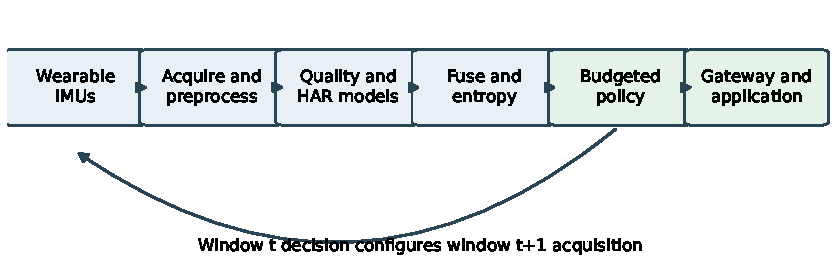
\includegraphics[width=0.92\textwidth]{figures/architecture.pdf}
\caption{End-to-end simulated AIoT architecture. The gateway decision at window $t$ can alter acquisition at $t+1$.}
\label{fig:architecture}
\end{figure*}

\section{Literature Survey and Gap}
Centaur uses denoising and multimodal fusion for incomplete HAR signals \cite{centaur}. Dong \emph{et al.} evaluate wearable sensor reliability through multiple criteria and evidential fusion \cite{dong}. Zuo \emph{et al.} combine sensor-level probabilities with self-reliability, discrepancy, and uncertainty \cite{zuo}. These approaches operate on acquired readings. AdaSense changes a wearable sensing configuration using an accuracy and power trade-off \cite{adasense}. Demirel \emph{et al.} address dynamic ECG sensor selection with a contextual bandit \cite{demirel}. CoSS selects sensors and sampling rates through trainable scores and pruning \cite{coss}. The gap identified in the six papers reviewed in our Part 1 report is an explicit combination of online signal-quality gating, predictive uncertainty, and a next-window sensing budget under injected faults. This is a scoped comparison, not a claim of priority over all literature.

Centaur's denoising autoencoder and attention-enhanced multimodal network target missing and noisy HAR streams \cite{centaur}. Its strength is a learned reconstruction and recognition pipeline across sensor channels. Its limitation for this question is timing: the corrupted measurements are already received before cleaning. Our system does not reproduce Centaur's architecture; instead, it asks whether an observable quality score can influence which channels are acquired later. Dong \emph{et al.} combine conflict and imprecision in a reliability analysis for body sensor networks \cite{dong}. That work motivates discounting weak sensor evidence, but its evidence-fusion machinery is distinct from our normalized probability average. Our implementation uses physically interpretable signal indicators so an injected dropout can be detected without consulting its test label.

Zuo \emph{et al.} evaluate each sensor's decision through self-reliability, discrepancy, and uncertainty before evidential fusion \cite{zuo}. Their method supports the value of sensor-specific decision streams, but its reliability includes validation-derived behavior and probability-level disagreement. Our controller uses a narrower runtime signal-quality definition and reuses fused entropy for an action at the next window. The difference matters: a prediction may be uncertain because two healthy sensors disagree, while a flatline can look spuriously confident. Neither quantity should be treated as a complete substitute for the other.

AdaSense demonstrates that activity-aware sensing configurations can reduce measured power on its wearable platform \cite{adasense}. It provides a precedent for pre-acquisition adaptation and stable configuration changes. Its setting centers on switching sensing modes for a wearable classifier, while our experiment explicitly injects IMU degradation and uses an estimated health gate. Demirel \emph{et al.} select ECG leads dynamically with a neural contextual bandit \cite{demirel}. That is a useful model of online resource allocation, but its cardiac task, lead geometry, and reward design do not transfer directly to three motion IMUs. Our simpler policy avoids learning a reward from test subjects, at the cost of hand-chosen thresholds.

CoSS jointly optimizes sensor modality and sampling rate through trainable scores followed by pruning \cite{coss}. It addresses data efficiency and model footprint, but its selected configuration is a product of training rather than a direct reaction to a transient stuck or missing sensor during a test stream. Together, the six studies separate three useful ideas: robust processing after data arrive, decision-level source discounting, and resource-aware sensing before acquisition. Our limited gap is their conjunction in one auditable fault-injection benchmark. Comparing their published metrics numerically with ours would be misleading because activities, subject splits, modalities, fault processes, and cost units differ.

\begin{table}[t]
\caption{Critical comparison of the six reviewed studies}
\centering\footnotesize
\begin{tabular}{p{0.14\columnwidth}p{0.34\columnwidth}p{0.36\columnwidth}}
\toprule Work & Main method & Relevance and limitation for this study \\
\midrule
Centaur \cite{centaur} & Denoising and multimodal HAR & Robustness after acquisition \\
Dong \cite{dong} & Multi-criteria reliability fusion & No pre-acquisition gating \\
Zuo \cite{zuo} & Triple reliability evaluation & Decision-level fusion of received data \\
AdaSense \cite{adasense} & Runtime sensing adaptation & No explicit fault-health estimate \\
Demirel \cite{demirel} & ECG lead selection bandit & Different sensing task and input \\
CoSS \cite{coss} & Sensor and rate optimization & Configuration selected through training \\
\bottomrule
\end{tabular}
\end{table}

\section{Dataset and Preprocessing}
PAMAP2 contains nine participants, 18 activity labels, three 100-Hz IMUs on the dominant wrist/hand, chest, and ankle, and a lower-rate heart-rate monitor \cite{pamap2}. The 54-column protocol files contain timestamp, activity ID, heart rate, and 17 values per IMU. This implementation selects the $\pm16g$ accelerometer and gyroscope axes from each IMU: zero-based columns 4--6 and 10--12 for hand, 21--23 and 27--29 for chest, and 38--40 and 44--46 for ankle. The always-on ``wrist'' node denotes the complete hand IMU's six chosen channels, not only its accelerometer. Labels 1--6 are used for a six-class feasibility study; activity 0 and other classes are excluded. This choice narrows the task and prevents direct comparison with full PAMAP2 benchmarks.

Per-subject windows have 256 samples (2.56 s) and stride 128 (50\% overlap). A window is retained when at least 80\% of samples have the majority label, and windows spanning timestamp gaps after filtering are rejected. Channel means and standard deviations are fit on training subjects only. The held-out subject is never used for fitting. Long natural gaps are imputed with zero after bounded interpolation; this choice can obscure native missingness, so fault detection results are limited to injected faults until raw missing masks are retained.

\section{System Methodology}
At window $t$, active IMUs produce signals $x_i(t)$. A sensor-specific random forest, or optional compact CNN--LSTM, yields a class probability vector $p_i(t)$ (Fig.~\ref{fig:fusion}). The baseline estimator combines missingness, flatline, first-difference noise, and distribution-shift penalties $q_{ij}(t)\in[0,1]$:
\begin{equation}
r_i(t)=\operatorname{clip}_{[0,1]}\left(1-\sum_j\alpha_jq_{ij}(t)\right).
\end{equation}
Weights $\alpha_j$ are normalized and set in the configuration file. A training-calibrated distribution-shift indicator is included as a bias/drift proxy. Its threshold has not yet been validated on official-data fault streams. The normalized weighted fusion is
\begin{equation}
p(k\mid t)=\frac{\sum_{i\in A_t}r_i(t)p_i(k\mid t)}{\sum_{i\in A_t}r_i(t)}.
\end{equation}
When the active total weight falls below 0.05, the implementation uses a uniform \emph{class prior} rather than trusting any sensor prediction; this produces high entropy and can prompt a new sensing configuration. Uncertainty is normalized entropy $u(t)=-\sum_{k=1}^Kp(k\mid t)\log p(k\mid t)/\log K$. The equal-weight acquisition and communication \emph{proxy} is $C(A_t)=\sum_{i\in A_t}c_i/\sum_i c_i$. It is neither joules nor measured battery power.

\begin{figure}[t]
\centering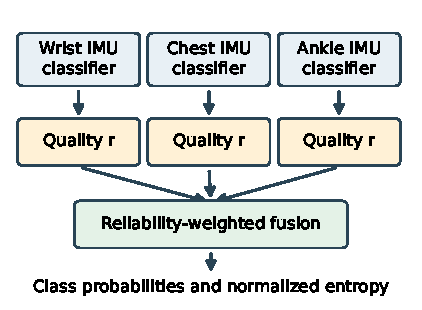
\includegraphics[width=\columnwidth]{figures/model_workflow.pdf}
\caption{Per-IMU classifiers and quality scores feed the fusion stage; inactive IMUs supply neither a current prediction nor a fresh quality score.}
\label{fig:fusion}
\end{figure}

The controller observes only active IMUs at $t$, then chooses $A_{t+1}$ (Fig.~\ref{fig:loop}). High entropy or low active-sensor reliability may activate an affordable optional IMU. Low entropy or detected failure may deactivate an optional IMU after a dwell period. The wrist anchor stays active. Inactive reliability is retained from its last observation, discounted by $0.98$ per unobserved window for candidate ranking, and refreshed by periodic probes; probing contributes to the cost proxy. A configured budget bounds the next active set. The evaluation must log masks, uncertainty, reliability, actions, and predictions per window before claiming policy behavior.

\begin{figure}[t]
\centering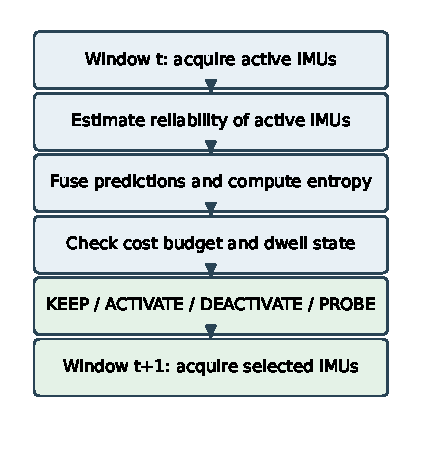
\includegraphics[width=\columnwidth]{figures/adaptive_policy.pdf}
\caption{Next-window control loop. Post-acquisition weighting and pre-acquisition selection have distinct effects.}
\label{fig:loop}
\end{figure}

\section{Implementation Details}
Three separate random forests provide subset-compatible predictions, one for each selected six-axis IMU. Each 256-sample window is summarized by 72 time-domain features: nine statistics for each of six channels and two vector magnitudes. The reduced-compute runs use 50 trees per IMU, depth at most 15, minimum leaf size two, balanced class weights, and seed 42. A comparison family uses two temporal convolutions (32 and 64 filters, kernel widths seven and five), max pooling, a unidirectional 64-unit LSTM, 0.3 dropout, and a six-class output. The reduced mode trains for up to five epochs with Adam at learning rate 0.001, batch size 64, and validation-based early stopping. Separate models mean an inactive IMU is not replaced by an invented current signal.

The quality score weights are 0.30 for missingness, 0.25 for flatline, 0.25 for first-difference noise, and 0.20 for a training-calibrated distribution shift. A reading below $r_{\rm low}=0.40$ is considered degraded by the controller. Entropy thresholds are $u_{\rm high}=0.65$ and $u_{\rm low}=0.35$. Each IMU has equal proxy weight; the budget is 0.667, which permits the wrist plus one optional IMU. The minimum dwell is four windows, and an inactive IMU is considered for a probe after 20 unobserved windows. These values are initial engineering choices, not validated physiological thresholds.

The test harness injects faults after training-only scaling into the held-out stream. Missing segments use NaN markers visible to the reliability estimator and converted to zero only inside classifiers that require finite features. Gaussian noise and drift magnitudes are therefore in standardized channel units, not physical acceleration or angular-rate units. The six configurations include separate dropout, intermittent blocks, noise, drift, flatline, and combined noise-plus-missingness. The same corrupted arrays are used by competing methods within a scenario. Offline batch caching accelerates scenario replay, but cached predictions from an inactive IMU are never passed to the controller or fusion. Such replay timing cannot be interpreted as deployment inference latency.

\section{Experimental Protocol}
The runner compares wrist only, wrist plus chest, all-sensor uniform fusion, all-sensor reliability-weighted fusion, and adaptive reliability-weighted fusion with shared per-sensor models. The reduced-compute full-fast mode performs leave-one-subject-out evaluation across the eight subjects with six-class data. Each fold uses the other subjects for fitting and a separate subject for CNN validation. The quick mode uses two development subjects and one held-out subject. Faults are injected only into held-out windows: complete or partial dropout, intermittent blocks, Gaussian noise, flatline, drift, and combined corruption. A standalone ablation replays a saved fold with one policy component changed at a time. Runs save input hashes and clean and moderate-dropout adaptive window logs. Report accuracy, macro precision, macro recall, macro F1, confusion matrices, fault-detection AUROC, active-node ratio, proxy cost, switches, and host latency from actual logs. Relative proxy reduction is $100(1-C_{\rm method}/C_{\rm all})\%$; macro-F1 degradation is $100(F1_{\rm clean}-F1_{\rm fault})$ percentage points.

A follow-up nested search reused each outer fold's training-only scaler and saved 50-tree random forests, and trained a 100-tree, depth-20, minimum-leaf-two candidate on that fold's six fitting subjects. Its seventh non-test subject selected the model using all-uniform fixed-six-class macro-F1 weighted across clean, moderate dropout, noise, and combined corruption (0.35, 0.25, 0.20, 0.20). The same validation subject selected among the original policy; a conservative policy with entropy thresholds 0.75/0.45, dwell 8, probe interval 40; and an early-reinforcement policy with thresholds 0.50/0.25, dwell 8, probe interval 12. The policy objective subtracted 0.10 times clean normalized cost and 0.02 times clean switches per window from that recognition score. The wrist anchor and 0.667 budget were fixed. Selection never read its own outer test subject. Selected choices were evaluated on six fault types at three severities, with seed 42 and deterministic per-subject fault streams. These subjects were previously examined in the historical run, so this is an exploratory nested follow-up rather than an external validation cohort.

\section{Results and Discussion}
\textbf{Provenance.} The main results come from run \texttt{full\_fast\_1792678712\_34ed82} using CRC-checked protocol files from the official UCI archive. Its manifest records input SHA-256 hashes. The eight usable subjects contribute 8,273 windows in total; each outer fold holds out one subject and trains/scales on the others with one separate validation subject. Reported spreads are standard deviations of eight held-out subject scores, not confidence intervals. Subject 109 is excluded because its official protocol file has labels 24 and 0 but no rows in the selected six-class task. Subject 103 has only four of the six selected classes, so macro-F1 across folds should be interpreted with differing held-out class support. A legacy repository quick run was excluded because it could have used synthetic data and mixed fixed numbers with measurements.

\begin{table}[t]
\caption{Historical clean eight-subject LOSO, random-forest fusion; macro-F1 uses labels observed in truth or prediction}
\centering\footnotesize
\begin{tabular}{lcc}
\toprule Configuration & Macro-F1 $\pm$ SD & Cost proxy \\
\midrule
Wrist only & $0.7850\pm0.1233$ & 0.33 \\
Wrist + chest fixed & $0.9150\pm0.0482$ & 0.67 \\
All IMUs, uniform & $0.8891\pm0.0726$ & 1.00 \\
All IMUs, reliability weighted & $0.8900\pm0.0726$ & 1.00 \\
Proposed adaptive & $0.8574\pm0.0861$ & 0.53 \\
\bottomrule
\end{tabular}
\label{tab:clean}
\end{table}

\begin{figure}[t]
\centering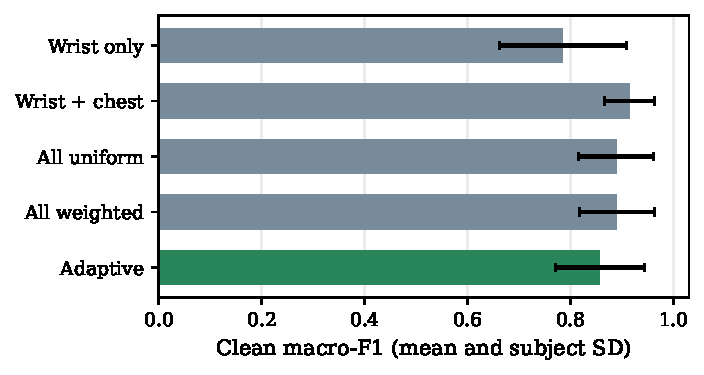
\includegraphics[width=\columnwidth]{figures/clean_comparison.pdf}
\caption{Clean recognition across eight held-out subjects. Error bars show subject-level standard deviation.}
\label{fig:clean}
\end{figure}

The controller's exact mean cost was 0.5281, a 47.2\% reduction in the \emph{normalized acquisition/communication proxy} relative to all IMUs active (Fig.~\ref{fig:tradeoff}). The logged masks show 930 sensor toggles over 8,273 windows (0.1124 toggles per window), including probes. On clean data (Fig.~\ref{fig:clean}), its observed-label mean macro-F1 was 3.2 percentage points below all-IMU uniform fusion and 5.8 points below the fixed wrist-plus-chest subset. The separate adaptive CNN--LSTM reached $0.8155\pm0.0698$ observed-label macro-F1 at cost 0.53. Thus, the fixed pair is the strongest clean comparator in this configuration, and the proposed method trades recognition for a lower proxy cost.

\begin{table}[t]
\caption{Moderate wrist-fault macro-F1, mean of eight held-out subjects}
\centering\footnotesize
\begin{tabular}{lccc}
\toprule Fault & All uniform & All weighted & Adaptive \\
\midrule
Dropout & 0.8501 & 0.8415 & 0.7919 \\
Intermittent & 0.8495 & 0.8411 & 0.7924 \\
Gaussian noise & 0.7690 & 0.8017 & 0.6522 \\
Flatline & 0.9006 & 0.9008 & 0.8339 \\
Drift & 0.8097 & 0.8140 & 0.6857 \\
Combined & 0.7758 & 0.8115 & 0.6883 \\
\bottomrule
\end{tabular}
\label{tab:fault}
\end{table}

All-sensor reliability weighting helped against the configured noise and combined faults; the adaptive budget constrained redundancy and generally reduced recognition. Moderate-dropout adaptive F1 was 0.7919, 6.6 percentage points below its own clean mean and 5.8 points below the all-sensor uniform method under the same fault. The injected missingness is explicit NaN, so detecting complete dropout is easier than detecting less visible drift. Across all configured faults, severities, and folds, the estimator's mean AUROC was 0.8882, while mean thresholded detection F1 was only 0.3402. The latter exposes missed faults despite low false-alarm rates. These are injected-fault metrics, not evidence of natural fault detection. Per-subject moderate-dropout adaptive F1 ranged from 0.4536 to 0.9491, indicating substantial heterogeneity. Desktop timing includes different batching across baselines, so it does not establish comparative embedded inference latency; no hardware joules were measured.

\begin{table}[t]
\caption{Policy ablation on subject 105; independently seeded fault replay}
\centering\scriptsize
\begin{tabular}{lcccc}
\toprule Variant & Clean F1 & Cost & Drop F1 & Noise F1 \\
\midrule
Standard & 0.754 & 0.645 & 0.742 & 0.546 \\
No reliability gate & 0.754 & 0.645 & 0.704 & 0.546 \\
No uncertainty control & 0.762 & 0.661 & 0.742 & 0.546 \\
No budget constraint & 0.840 & 0.918 & 0.850 & 0.793 \\
Uniform fusion & 0.761 & 0.645 & 0.787 & 0.455 \\
No dwell & 0.754 & 0.644 & 0.742 & 0.546 \\
\bottomrule
\end{tabular}
\label{tab:ablation}
\end{table}

The ablation replay in Table~\ref{tab:ablation} isolates one controller or fusion choice at a time on subject 105. Removing the budget raises recognition but nearly restores all-sensor cost; removing reliability gating worsens moderate-dropout F1 in this replay. Uniform fusion helps this particular dropout case but harms the seeded noise case. Dwell removal makes little difference to F1 here, so a claim that dwell improves recognition is unsupported. The replay's independently seeded noise stream differs from the main grid's sequential random stream, so its exact fault F1 values should not be compared cell-for-cell with Table~\ref{tab:fault}.

\subsection{Nested Optimization Follow-up}
The follow-up's fixed-six-class metric assigns zero F1 to a selected class absent from a held-out fold, unlike the historical observed-label macro-F1. This distinction affects subject 103, which lacks two selected classes; values from the two protocols are not directly interchangeable. The original 50-tree model and original policy were replayed on the new evaluation stream, reproducing the historical clean observed-label mean 0.8574, cost 0.5281, and 930 mask-derived toggles. Table~\ref{tab:nested_clean} compares every method with the fixed-six-class definition. Validation chose the 100-tree model in six of eight folds and changed the policy in three. The selected method reduced switching to 858 toggles (0.1037 per window), but clean macro-F1 fell by 2.0 percentage points relative to the replayed original at nearly the same sensing-cost proxy.

\begin{table}[t]
\caption{Nested eight-subject clean evaluation; fixed-six-class macro-F1, mean $\pm$ subject SD}
\centering\scriptsize
\begin{tabular}{lcc}
\toprule Configuration & Macro-F1 & Cost proxy \\
\midrule
Original RF + original policy & $0.8428\pm0.1158$ & 0.5281 \\
Selected RF + original policy & $0.8418\pm0.1168$ & 0.5278 \\
Selected RF + selected policy & $0.8227\pm0.1194$ & 0.5310 \\
Wrist + chest, selected RF & $0.8574\pm0.1116$ & 0.6667 \\
All uniform, selected RF & $0.8533\pm0.1108$ & 1.0000 \\
All weighted, selected RF & $0.8540\pm0.1114$ & 1.0000 \\
\bottomrule
\end{tabular}
\label{tab:nested_clean}
\end{table}

\begin{figure}[t]
\centering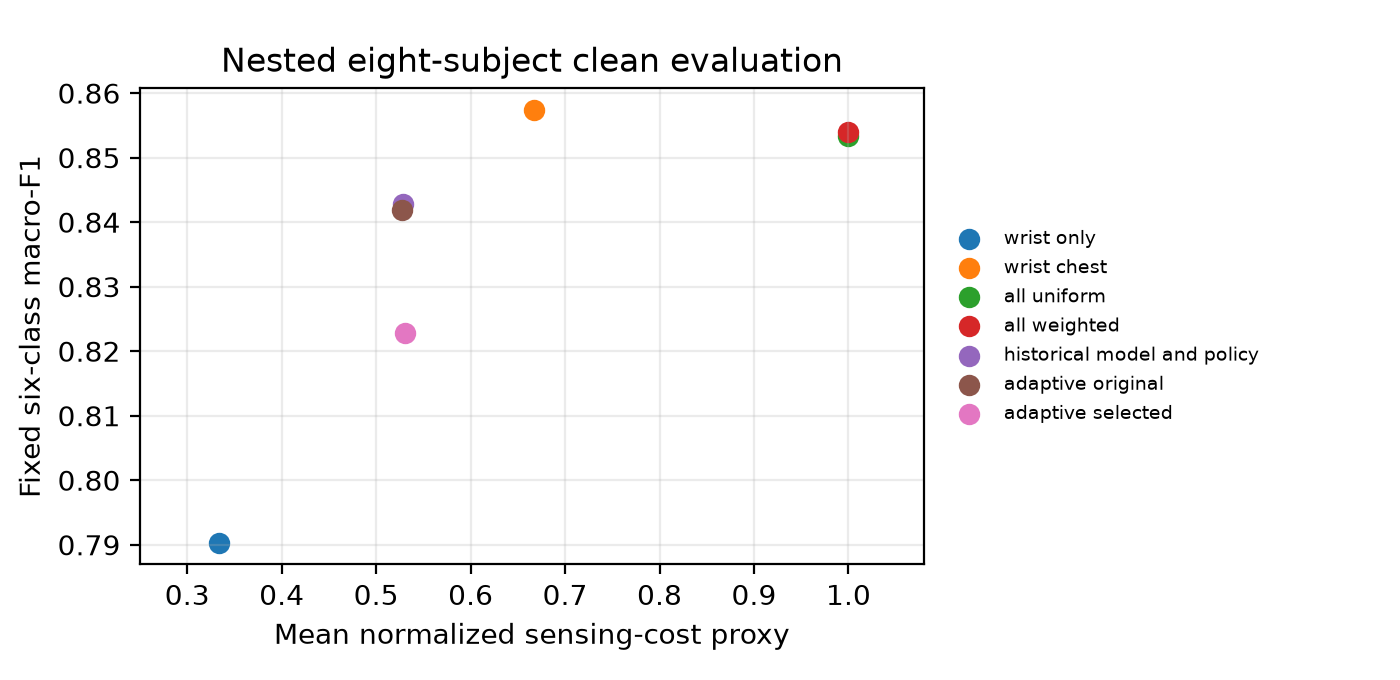
\includegraphics[width=\columnwidth]{figures/nested_cost_tradeoff.png}
\caption{Fixed-six-class clean macro-F1 against normalized sensing-cost proxy in the nested follow-up. Points are eight-subject means, not measured energy.}
\label{fig:nested_tradeoff}
\end{figure}

At moderate wrist dropout, fixed-six macro-F1 was 0.7559 for the selected adaptive method, 0.8217 for all-uniform, and 0.8112 for all-weighted fusion. For moderate Gaussian noise the scores were 0.6471, 0.7630, and 0.7922; for moderate combined corruption they were 0.6766, 0.7661, and 0.7978, respectively. The full six-fault, three-severity grid is saved with the run. Figure~\ref{fig:nested_dropout} shows the selected method below both all-sensor comparators at each tested dropout severity. The cost budget limits redundancy under faults. The largest clean loss occurred on subject 105: 0.7319 selected versus 0.8474 original under the fixed-six metric. Single-subject inner validation did not reliably predict another person's performance. The original 50-tree configuration therefore remains the recommended tested setting; no significance or broad generalization claim follows from these eight folds.

\subsection{Subject-Level Error Analysis}
Table~\ref{tab:subject_nested} exposes the held-out scores behind the means in Table~\ref{tab:nested_clean}. Each row compares the validation-selected model and policy with the original 50-tree model and original policy replayed on the \emph{same} subject, using the same fixed-six-class definition. The table reports every test subject rather than selecting a favorable fold. Subjects 102 and 103 are unchanged because inner validation retained both original choices. Subject 104 is the only fold with a positive selected-minus-original clean difference, and that difference is 0.0038. The largest decline, 0.1155 on subject 105, exceeds the small gains elsewhere and materially affects the eight-subject mean. Subject 103 has only four true classes in the selected six-class task; assigning zero F1 to the other two classes lowers both configurations equally in this within-subject comparison.

\begin{table}[t]
\caption{Nested clean fixed-six macro-F1 by held-out subject. The difference is selected minus replayed original; $n$ is the number of test windows.}
\centering\footnotesize
\begin{tabular}{r r c c r}
\toprule Subject & $n$ & Original & Selected & Difference \\
\midrule
101 & 1080 & 0.8112 & 0.7864 & $-0.0248$ \\
102 & 1068 & 0.9302 & 0.9302 & $+0.0000$ \\
103 & 778 & 0.5875 & 0.5875 & $+0.0000$ \\
104 & 991 & 0.7592 & 0.7629 & $+0.0038$ \\
105 & 1192 & 0.8474 & 0.7319 & $-0.1155$ \\
106 & 1081 & 0.9266 & 0.9121 & $-0.0145$ \\
107 & 955 & 0.9244 & 0.9189 & $-0.0056$ \\
108 & 1128 & 0.9555 & 0.9520 & $-0.0035$ \\
\bottomrule
\end{tabular}
\label{tab:subject_nested}
\end{table}

The selection outcomes help localize the trade-off. The 100-tree candidate was chosen in six folds, but selected forests paired with the \emph{original} policy reached 0.8418 mean clean F1 at cost 0.5278. Pairing those forests with the selected policies yielded 0.8227 at cost 0.5310. Thus, changing the policy after model selection coincided with most of the observed aggregate clean loss; model-policy interactions prevent a stronger causal attribution. On subject 105, the conservative policy reduced its clean proxy cost from 0.5159 to 0.4502 and its switches from 169 to 133, while fixed-six clean F1 fell from 0.8474 to 0.7319. On subject 104, early reinforcement raised the cost from 0.5742 to 0.6199 for a 0.0038 F1 gain. These paired outcomes show why a single validation subject is an unstable guide to the recognition--cost trade-off on another person.

\subsection{Reproducibility and Measurement Boundaries}
The nested run records a clean test and 18 faulted tests per held-out fold: six fault constructions at mild, moderate, and severe settings. Its protocol records the model candidates, policy thresholds, objective weights, and random seed. The saved per-fold records contain the chosen model and policy, validation scores, test metrics, and cost traces; clean and moderate-dropout adaptive logs retain predictions and active masks window by window. Recomputing F1 from those predictions and toggles from adjacent masks checks the aggregate independently of its CSV export. The result figures are generated from the saved records rather than drawn from the manuscript's rounded values.

The cost $C(A_t)$ counts active IMUs with equal weights. It omits sensor warm-up, radio retransmissions, computation, battery chemistry, and the cost of a control message. A mask toggle is therefore a stability indicator, not a measured switching-energy penalty. Likewise, fault-detection AUROC evaluates the injected labels supplied by the simulator; thresholded detection F1 reveals that a high ranking score does not guarantee reliable alarms at the chosen threshold. Host-side replay time includes caching and batching and cannot establish latency on a wearable gateway. These boundaries are important when interpreting the 47.2\% proxy reduction: it is a reproducible property of the logged masks, while physical energy savings remain a future measurement.

\begin{figure}[t]
\centering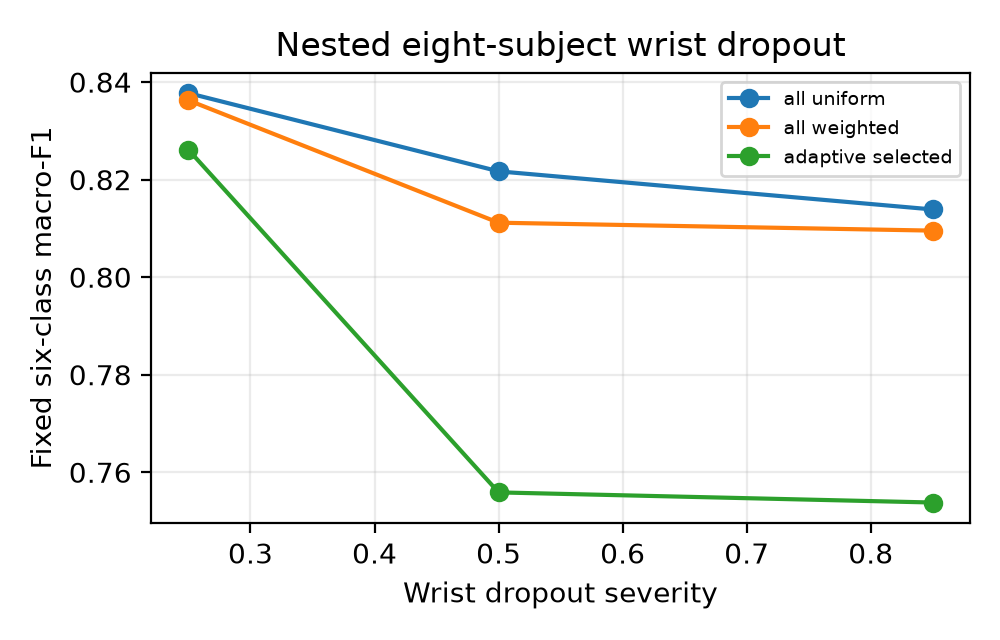
\includegraphics[width=\columnwidth]{figures/nested_dropout_severity.png}
\caption{Nested eight-subject fixed-six macro-F1 across mild, moderate, and severe simulated wrist dropout.}
\label{fig:nested_dropout}
\end{figure}

\begin{figure}[t]
\centering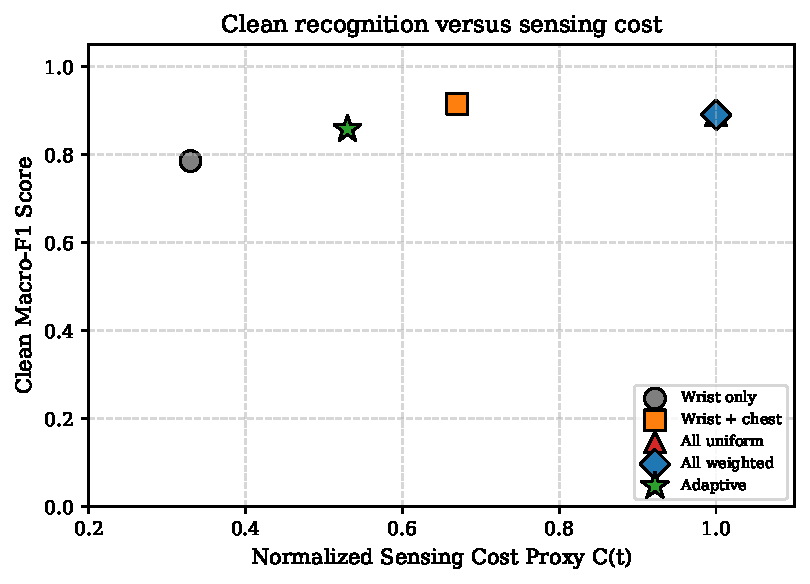
\includegraphics[width=\columnwidth]{figures/fig7_cost_vs_macro_f1.pdf}
\caption{Mean clean recognition versus normalized sensing-cost proxy across eight held-out subjects.}
\label{fig:tradeoff}
\end{figure}

\begin{figure}[t]
\centering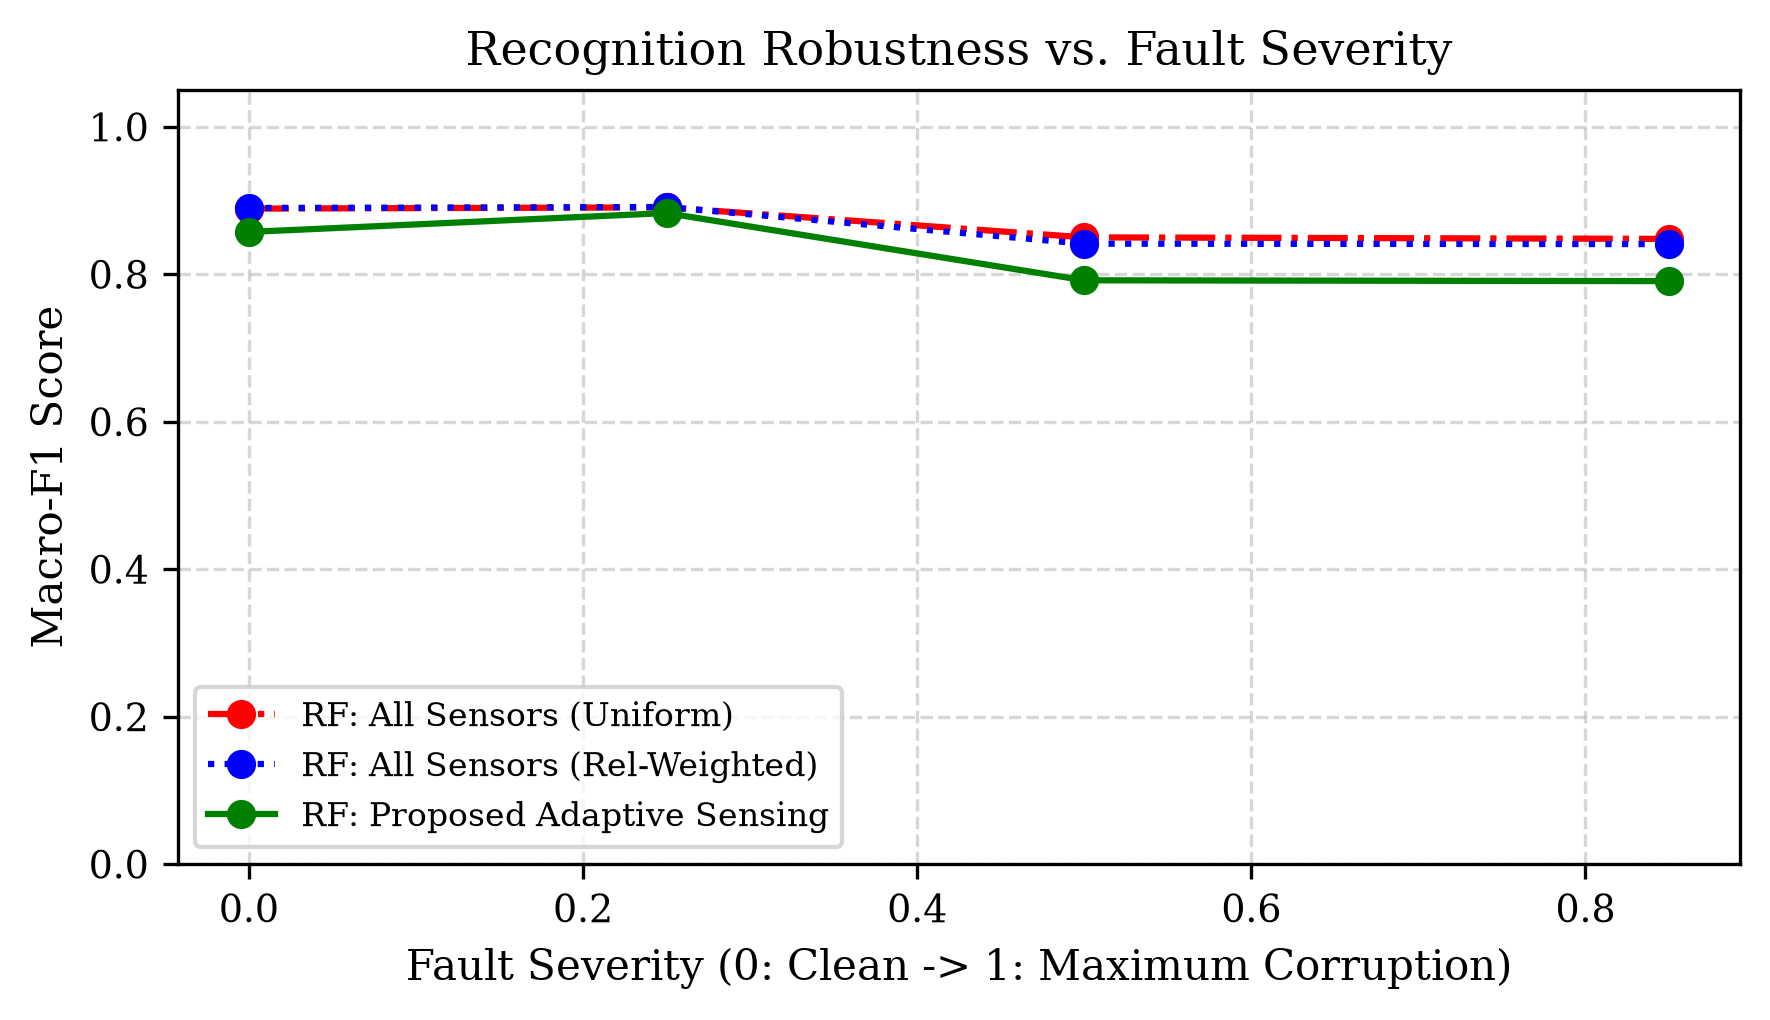
\includegraphics[width=\columnwidth]{figures/fig5_macro_f1_vs_severity.png}
\caption{Mean macro-F1 under wrist dropout severity across eight held-out subjects, including the clean reference.}
\label{fig:severity}
\end{figure}

\section{Limitations and Conclusion}
This implementation is a simulation over prerecorded IMU streams; physical node scheduling, radio energy, and clinical generalization are unmeasured. The eight-subject historical evaluation shows a 47.2\% reduction in a normalized sensing-cost proxy with lower clean and faulted recognition than the strongest fixed comparator. The nested search did not improve the held-out recognition--cost trade-off and illustrates unstable transfer from one validation person to another. Reliability weighting is more useful under some injected analog faults than under explicit missingness. Thresholds and cost weights require hardware-informed calibration; switching overhead may erode real savings. Future work should test calibrated energy, natural failures, more robust multi-subject inner validation, all available activity classes, richer uncertainty control, and a broader set of subjects and devices. The required institutional similarity report and group presentation remain separate submission steps.

\bibliographystyle{IEEEtran}
\bibliography{references}
\end{document}
